\documentclass{bioinfo}
\copyrightyear{2020} \pubyear{2020}

\access{Advance Access Publication Date: Day Month Year}
\appnotes{Manuscript Category}

\begin{document}
\firstpage{1}

\subtitle{Sequence analysis}

\title[short Title]{AttCRISPR : an spacetime interpretable model for sgRNA efficiency prediction
}
\author[Sample \textit{et~al}.]{Corresponding Author\,$^{\text{\sfb 1,}*}$, Co-Author\,$^{\text{\sfb 2}}$ and Co-Author\,$^{\text{\sfb 2,}*}$}
\address{$^{\text{\sf 1}}$Department, Institution, City, Post Code, Country and \\
$^{\text{\sf 2}}$Department, Institution, City, Post Code,
Country.}

\corresp{$^\ast$To whom correspondence should be addressed.}

\history{Received on XXXXX; revised on XXXXX; accepted on XXXXX}

\editor{Associate Editor: XXXXXXX}

\abstract{\textbf{Motivation:} More and more higher specificities Cas9 variants are developed to avoid the off-target effect, which bring a significant volume of experimental data. 
Conventional machine learning performance poorly on these datasets, while model based on deep learning are often lack of interpretability, which makes it difficult for researchers to understand its decisions. 
Moreover, neither the deep learning based model with existing structure can not satisfy enough precision at such huge datasets.\\
\textbf{Results:} To overcome it, we design and implement AttCRISPR, a deep learning based model to predict the on-target activity. 
Our model was trained and tested on the biggest dataset, DeepHF dataset, as far as we know for performance evaluation. 
AttCRISPR achieves the best performance on DeepHF dataset, yielding an average spearman value of 0.99\%, 0.99\%, 0.99\% (corresponding to WT-SpCas9, eSpCas9(1.1), SpCas9-HF1) under tenfold shuffled validation. 
In addition, another advantage of AttCRISPR over other well-perform methods is that it is intrinsic interpretable and does not rely on other post hoc explanations techniques. 
In this paper, We design a set of algorithm to reveal the biological significance of the decision maked by AttCRISPR from the global and local perspectives at sgRNA overall level and nucleotide level.\\
\textbf{Availability:} The example code are available at \href{https://github.com/South-Walker/AttCRISPR}{https://github.com/South-Walker/AttCRISPR}\\
\textbf{Contact:} \href{xlm@xiaoliming96.com}{xlm@xiaoliming96.com}\\
\textbf{Supplementary information:} Supplementary data are available at \textit{Bioinformatics}
online.}

\maketitle

\section{Introduction}

Clustered regularly interspaced short palindromic repeats (CRISPR) / CRIPSR associated protein 9 (Cas9) systems is preferred over other biological research and human medicine technologies now, beacuse of it's efficiency, 
 robustness and programmability.  Cas9 nucleases can be directed by short guide RNAs (sgRNAs) to introduce site-specific DNA double-stranded breaks in target, 
 so to enable editing site-specific within the mammalian genome \citep{jinek2012a,cong2013multiplex,mali2013rnaguided}. CRISPR/Cas9, to a large extent, has developed genetic therapies at the cellular level, 
 while there are still severe medical disadvantage even now which has greatly hindered the further clinical application of the CRISPR/Cas9 systems. 
 One of these disadvantage is due to point mutations caused by off-target effects \citep{rubeis2018risks,kang2016introducing,ishii2017reproductive,liang2015crispr/cas9-mediated}. 
 To overcome this disadvantage, a solution is to engineer CRISPR/Cas9 with higher specificities. 
 That's why more and more higher specificities Cas9 variants, such as enhanced SpCas9 (eSpCas9(1.1)), 
 Cas9-High Fidelity (SpCas9-HF1) \citep{ishii2017reproductive,slaymaker2016rationally}, hyper-accurate Cas9 (HypaCas9) \citep{kleinstiver2016high-fidelity}, 
 been developed and bring a significant volume of experimental data, that is to say researchers have to face the difficulty of analyzing such huge and heterogeneous data.

The activity of chosen sgRNA sequence determines the success of genome editing, however distinctly fluctuant behaviors have been observed for the performance of different sgRNAs, even in the same Cas9 system.
 Some optimum sgRNAs can hit almost all targers alleles, while anothers don't even show activity \citep{wang2019optimized}.
 This fact indicates that it's meaningful to explore an efficient approaches to guide sgRNA design. 


In practice, there have been a number of application and toolkit applied in this task. In the earlier studies, methods in silico are categorized into three types: 
 (1) alignment-based, (2) hypothesis-driven and (3) learning-based \citep{chuai2018deepcrispr}. 
 Recently we noticed that the last type of method seems to be getting more attention because of huger and huger data set \citep{liu2019computational}. 

Learning-based method, which designed to predict the activity of sgRNAs, is essentially a computational model built by machine learning algorithm, not only conventional machine learning but also deep learning algorithm. 
 Some studies on HT\_ABE and HT\_CBE have shown that deep learning based models often outperformed conventional machine learning, when the number of sgRNAs in the data set reached a certain level \citep{Song2020,kim2018deep,kim2019spcas9}. 
 Per contra, conventional machine learning algorithms, such as linear regression, logistic regression and the decision tree, are often more interpretable due to the fewer parameters and clearer mathematical assumptions. 
 In short, what was needed for developer is to trade-off accuracy and interpretability. 
 \citeauthor{MuhammadRafid2020} consider deep-learning-based models as black boxs and believe they lack interpretability, 
 motivated by the empirical assertion, they turn to build a model based conventional machine learning to compete with state of the art deep learning models \citep{MuhammadRafid2020}. 
 On the other hand, input perturbation based feature importance analysis become a preferred components to reveal the importance of features in deep learning models. 
 \citeauthor{Liu2019} use a sliding window of length 2 to extract dimeric as input and rank the position of dimeric by contribution to final output \citep{Liu2019}. 
 One regret is that subject to the processing of the input sgRNA sequence, their analysis can not exactly on the nucleotide class. Further, SHAP, one of the most prominent of model explain techniques, has been widely used to understand the decision made by the model. 
 \citeauthor{wang2019optimized} develope DeepHF, a deep learning based model, and use Deep SHAP to revealed nucleotide contributions \citep{wang2019optimized}. 
 Deep SHAP is a compositional approximation of SHAP values since it is challenged to computate SHAP values exactly, especially for a complex deep neural networks \citep{lundberg2017a}. 
 In our understanding, the method based on input perturbation often requires better generalization ability of the model (even for artificial ridiculous noise data). 
 Moreover, recent work indicates that model explain techniques, which based post hoc explanations techniques and input perturbations, could be fooled to generate meaningless explanations instead of reflecting the underlying biases \citep{slack2019fooling}, in other word, they could be unreliable and misleading, even on model with excellent performance. 
 In addition, as far as we know, all the interpretable deep learning models today can only analyze the preference of on-target activity (or off-target probability) on specific nucleotide species and position (for example, the guanine (G) adjacent to PAM has a positive effect on sgRNA activity), which we'll call the first-order preference in our paper.  
 However they didn't analyzed the preference for sgRNA at the overall level, which we'll call the second-order preference in our paper (for example, could a thymine (T) at 2 bases upstream of the G adjacent to PAM affect the degree of preference for the G?)
 We agree that base on the first-order influence and Bayesian formula can obtain the second-order preference in a statistical sense. However, it is obviously time-consuming task with exponential time complexity.
 In light of the above, we believe it is essential to develope a model which can not only match deep learning based model in performance, but also be comparable to conventional machine learning algorithms in interpretability.

\begin{figure}[!tpb]%figure2
    \centerline{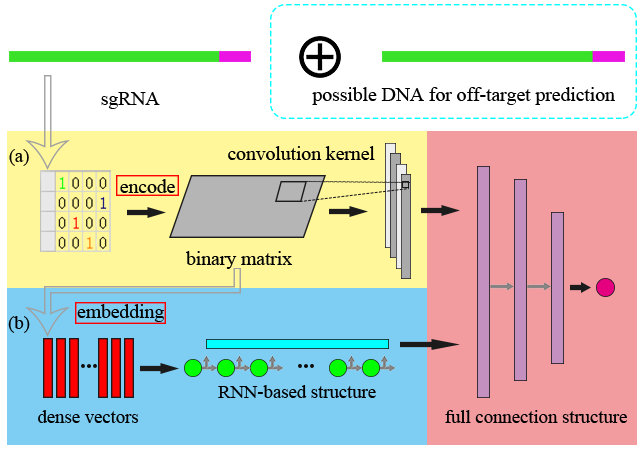
\includegraphics[scale=0.5]{category.png}}
    \caption{Two categories of the deep learning models used in sgRNA related task. 
    (a) Model work in spatial domain. (b) Model work in temporal domain.}\label{fig:01}
\end{figure}
    
Deep neural network has shown its power in the study of CRISPR/Cas9 and its improved Systems \citep{liu2019computational}. 
 Most of the deep neural network existing are the combination of recurrent neural network (RNN), convolutional neural network (CNN), fully connected neural network (FNN), and their variants. 
 We found that the deep learning models used in sgRNA on-target activity (even for off-target effect) prediction tasks in recent years can be divided into the following two categories according to the encoding approach of the sgRNA sequence (sgRNA-DNA sequence pair, for off-target effect prediction):

\begin{enumerate}
    \item Methods in spatial domain. 
    Some previous studies have used model based CNN to predict gRNA on-target activity or off-target effects \citep{lin2018off-target,kim2018deep,chuai2018deepcrispr}. 
    They process sgRNA base sequence inputs with the help of one-hot encoding idea. 
    In other words, they regard it as two-dimensional image data, and use convolution layer to extracte potential features in spatial domain, 
    It is worth noting that \citeauthor{zhang2020c-rnncrispr:} adds bidirectional gated recurrent unit (BGRU, in short), a RNN variant, after pooling layer of classic CNN network \citep{zhang2020c-rnncrispr:}. 
    Our explanation is that BGRU assists CNN to extract spatial features in one dimension, under this belief it belong to this category. 
    \item Methods in temporal domain. 
    Although RNN-based network have been shown effective to improve the performance of the model with temporal sequential input, especially in natural language processing and sequential recommendation\citep{huang2018improving}, 
    RNN be not used for gRNA activity prediction, until recently \citep{wang2019optimized,liu2020deep,Liu2019}. 
    They consider the nucleotides(can also dimer or polymer) in the sgRNA sequence as word, and the sgRNA sequence itself as a sentence (from 5' to 3'), then a trainable matrix (could be either supervised or unsupervised) is used to project the word to the dense real-valued space. 
    This technology is called embedding, which generates the base embedding. RNN further encoding the base embedding into a sequence of hidden state vector. 
    Specially, \citeauthor{Liu2019} use RNN and CNN in parallel to extract features in base embedding \citep{Liu2019}. 
    However, base embedding is not spatially interpretable (different from one-hot encode), and they have no way to further explore the correlation between CNN and RNN output. 
    Almost all RNN based models used in sgRNA on-target activity or off-target effect flatten the hidden state vector into a one-dimensional vector as the input of the fully connected layer. 
    It is a pity that the temporal sequential dependency of hidden state vector are rarely noticed. 
    To summarise, RNN has limited representation power in capturing spatial feature. Furthermore, hidden state vector representation is usually hard to understand and explain.
\end{enumerate}

Attention mechanism has demonstrated its power in Natural Language Processing, Statistical Learning, Speech and Computer Vision \citep{chaudhari2019an}. 
 It makes model tends to focus selectively on parts of the input which is help in performing the task effectively. 
 Previous observation have shown that Cas9 preferentially binds sgRNAs containing purines but not pyrimidines \citep{wang2014genetic} and multiple thymine in the spacer impairing sgRNA activity \citep{wu2014genome-wide}, 
 that is to say some specific nucleotide and base position need more attention compared to others. 
 The above is the premise of introducing attention mechanism. Strictly speaking, we are not the first to bring attention mechanisms into this field. 
 The most similar approach to ours is the work based on transformer by \citeauthor{Liu2019}. 
 They use transformer, a components based on attention mechanism, instead of RNN to improve the ability of temporal feature extraction, hence, enhance the performance of their model \citep{Liu2019,vaswani2017attention}. 
 In our work,the interpretability benefit from attention mechanism is more focused.


In this paper, our main contributions are as follows:\vspace*{1pt}

\begin{itemize}
    \item Present a novel deep-learning-based model, which can extract potential feature representation of sgRNA sequence in both spatial and temporal domain parallelly. 
    Finally, the ensemble learning method is used to combine the two to achieve better performance than other models.
    It doesn't belong to any of the above categories of existing approaches.
    \item Introduce attention mechanism into our model. 
    As a result, It does not need post hoc explanations techniques based on input perturbation to explain itself. 
    It is intrinsic interpretable in both temporal and spatial domains.
    In the spatial domain it's at the nucleotide level, in our word, first-order interpretable, 
    while at the overall level in the temporal domain, in our word, second-order interpretable. 
    Thus, it is transformed from a black box to an intrinsically interpretable model with the performance of deep learning based model. 
    \item Throught abation analysis and testing a series of possible network structure, 
    we find there are multiple components and strategy can improve the performance of our model and constructed AttCRISPR, 
    which could outperform the current state-of-the-art tool on deepHF dataset.\vspace*{1pt}
\end{itemize}

\section{Materials and methods}

\subsection{Sequence and biological features embedding}

Text Text Text Text Text Text  Text Text Text Text Text Text Text
Text Text  Text Text Text Text Text Text.

\subsubsection{Spatial sequence embedding}

Text  Text 

\subsubsection{Temporal sequence embedding}

Text

\subsubsection{biological features embedding}

Text

\subsection{Neural network architecture}

Text

\subsubsection{Attention module and model in spatial domain}

Text

\subsubsection{Attention module and model in temporal domain}

Text

\subsubsection{Ensemble method boosting model}

Text

\subsection{Datasets and current prediction algorithms}

text

\subsection{Experiments}

text

{\ldots}{\ldots} text follows.
\begin{equation}
\sum \text{\it x}+ \text{\it y} =\text{\it Z}\label{eq:01}\vspace*{-10pt}
\end{equation}

%\enlargethispage{12pt}
\begin{methods}
\section{Results}

Text Text Text Text Text Text  Text Text Text Text Text Text Text
Text Text  Text Text Text Text Text Text.
Figure~2\vphantom{\ref{fig:02}} shows that the above method  Text
Text Text Text  Text Text Text Text Text Text  Text Text.
\citealp{Boffelli03} might want to know about  text text text text
text\vspace*{1pt}

Figure~2\vphantom{\ref{fig:02}} shows that the above method  Text
Text Text Text  Text Text Text Text Text Text  Text Text.

\subsection{This is subheading}

Text Text Text Text Text Text  Text Text Text Text Text Text Text
Text Text  Text Text Text Text Text Text.
Figure~2\vphantom{\ref{fig:02}} shows that the above method  Text
Text Text Text  Text Text Text Text Text Text  Text Text.
\citealp{Boffelli03} might want to know about  text text text text

\subsubsection{This is subsubheading}

Text Text Text Text Text Text  Text Text Text Text Text Text Text

Figure~2\vphantom{\ref{fig:02}} shows that the above method  Text
Text Text Text  Text Text Text Text Text Text  Text Text.
\citealp{Boffelli03} might want to know about  text text text.

\enlargethispage{6pt}

Text Text Text Text Text Text  Text Text Text Text Text Text Text
Text Text  Text Text Text Text Text Text.
Figure~2\vphantom{\ref{fig:02}} shows that the above method  Text
Text Text Text  Text Text Text Text Text Text  Text Text.
\citealp{Boffelli03} might want to know about  text text text text
Text Text Text Text Text Text  Text Text Text Text Text Text Text

\begin{table}[!t]
\processtable{This is table caption\label{Tab:01}} {\begin{tabular}{@{}llll@{}}\toprule head1 &
head2 & head3 & head4\\\midrule
row1 & row1 & row1 & row1\\
row2 & row2 & row2 & row2\\
row3 & row3 & row3 & row3\\
row4 & row4 & row4 & row4\\\botrule
\end{tabular}}{This is a footnote}
\end{table}

\end{methods}

\begin{figure}[!tpb]%figure1
\fboxsep=0pt\colorbox{gray}{\begin{minipage}[t]{235pt} \vbox to 100pt{\vfill\hbox to
235pt{\hfill\fontsize{24pt}{24pt}\selectfont FPO\hfill}\vfill}
\end{minipage}}
%\centerline{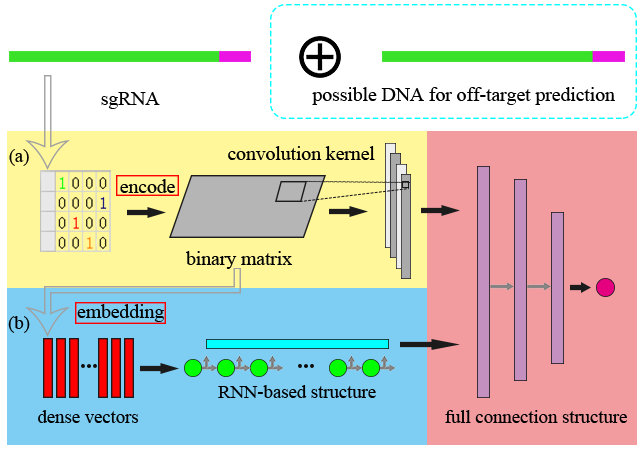
\includegraphics[scale=0.6]{category.png}}
\caption{Caption, caption.}\label{fig:02}
\end{figure}

Text Text Text Text Text Text  Text Text Text Text Text Text Text
Text Text  Text Text Text Text Text Text.
Figure~2\vphantom{\ref{fig:02}} shows that the above method  Text
Text Text Text  Text Text Text Text Text Text  Text Text.
\citealp{Boffelli03} might want to know about  text text text text
Text 


\subsection{Test1}

Text Text Text Text Text Text  Text Text Text Text Text Text Text
Text Text  Text Text Text Text Text Text.
Figure~2\vphantom{\ref{fig:02}} shows that the above method  Text
Text Text Text  Text Text Text Text Text Text  Text Text.
\citealp{Boffelli03} might want to know about  text text text text





\section{Discussion}

Text Text Text Text Text Text  Text Text Text Text Text Text Text
Text Text  Text Text Text Text Text Text.
Figure~2\vphantom{\ref{fig:02}} shows that the above method  Text
Text Text Text  Text Text Text Text Text Text  Text Text.
\citealp{Boffelli03} might want to know about  text text text text
Text Text Text Text Text Text  Text Text Text Text Text Text Text.



Table~\ref{Tab:01} shows that Text Text Text Text Text  Text Text
Text Text Text Text. Figure~2\vphantom{\ref{fig:02}} shows that
the above method Text Text. Text Text Text  Text Text Text Text
Text Text. Figure~2\vphantom{\ref{fig:02}} shows that the above
method Text Text. Text Text Text  Text Text Text Text Text Text.
Figure~2\vphantom{\ref{fig:02}} shows that the above method Text
Text.





%%%%%%%%%%%%%%%%%%%%%%%%%%%%%%%%%%%%%%%%%%%%%%%%%%%%%%%%%%%%%%%%%%%%%%%%%%%%%%%%%%%%%
%
%     please remove the " % " symbol from \centerline{\includegraphics{fig01.eps}}
%     as it may ignore the figures.
%
%%%%%%%%%%%%%%%%%%%%%%%%%%%%%%%%%%%%%%%%%%%%%%%%%%%%%%%%%%%%%%%%%%%%%%%%%%%%%%%%%%%%%%






\section{Conclusion}

(Table~\ref{Tab:01}) Text Text Text Text Text Text  Text Text Text
Text Text Text Text Text Text  Text Text Text Text Text Text.
Figure~2\vphantom{\ref{fig:02}} shows that the above method  Text
Text Text Text  Text Text Text Text Text Text  Text Text.
\citealp{Boffelli03} might want to know about  text text text text
Text Text Text Text Text Text  Text Text Text Text Text Text Text
Text Text  Text Text Text Text Text Text.
Figure~2\vphantom{\ref{fig:02}} shows that the above method  Text
Text Text Text  Text Text Text Text Text Text  Text Text.
\citealp{Boffelli03} might want to know about  text text text text
Text Text Text Text Text Text Text Text Text Text Text Text Text

Figure~2\vphantom{\ref{fig:02}} shows that the above method  Text
Text Text Text  Text Text Text Text Text Text  Text Text.
\citealp{Boffelli03} might want to know about  text text text text

\begin{enumerate}
\item this is item, use enumerate
\item this is item, use enumerate
\item this is item, use enumerate
\end{enumerate}

Text Text Text Text Text Text Text Text Text Text Text Text Text
Text Text Text Text Text Text Text Text.
Figure~2\vphantom{\ref{fig:02}} shows\vadjust{\pagebreak} that the
above method  Text Text Text Text Text Text Text Text Text Text
Text Text.  \citealp{Boffelli03} might want to know about text
text text text Text Text Text Text Text Text  Text Text Text Text
Text Text Text Text Text Text Text Text Text Text Text.
Figure~2\vphantom{\ref{fig:02}} shows that the above method  Text
Text Text Text Text Text Text Text Text Text  Text Text.
\citealp{Boffelli03} might want to know about text text text text
Text Text Text Text Text Text  Text Text Text Text Text Text Text
Text Text Text Text Text Text Text\break Text.

Figure~2\vphantom{\ref{fig:02}} shows that the above method  Text
Text Text Text\vspace*{-10pt}


\section*{Acknowledgements}

Text
text text text\vspace*{-12pt}

\section*{Funding}

This work has beenText  Text Text.\vspace*{-12pt}

\bibliographystyle{natbib}
%\bibliographystyle{achemnat}
%\bibliographystyle{plainnat}
%\bibliographystyle{abbrv}
%\bibliographystyle{bioinformatics}
%
%\bibliographystyle{plain}
%
\bibliography{document}

\end{document}
